% Generated using the supplied basilisk_i18n style; content: Basilisk Systems P.S.A. agreement + comments/graphics; coded terminology: Diana49, WRA, unia erebu.
% !TeX program = pdflatex

\documentclass[12pt,a4paper]{report}
\usepackage{basilisk_i18n}
\usepackage{lmodern}
\usepackage{microtype}
\usepackage{setspace}
\usepackage{parskip}
\usepackage[most]{tcolorbox}
\usepackage{tikz}
\usetikzlibrary{positioning,arrows.meta,shapes.geometric,calc}
\usepackage{needspace}
\usepackage{tabularx}

\BusinessPlanCompany{Basilisk Systems}
\BusinessPlanWatermarkText{Basilisk Systems}
\BusinessPlanWatermarkColor{black!6}
\BusinessPlanWatermarkFontSize{38}{46}
\BusinessPlanWatermarkAngle{38}
\BusinessPlanAuthorsText{Basilisk Systems --- dokument roboczy dla założycieli}
\BusinessPlanConfidentialText{Dokument roboczy --- komentarze nie stanowią tekstu umowy}
\BusinessPlanFooterText{Basilisk Systems --- umowa P.S.A. / tekst umowy + komentarze}
\BusinessPlanVersionText{Wersja robocza}

\setstretch{1.18}
\setlist[itemize]{topsep=0.2em,itemsep=0.15em,parsep=0.1em,leftmargin=2.0em}
\setlist[enumerate]{topsep=0.25em,itemsep=0.18em,parsep=0.1em,leftmargin=2.2em}
\setlength{\parindent}{0pt}
\setlength{\parskip}{0.55em}
\renewcommand{\arraystretch}{1.18}

\newcounter{paragraf}
\newcommand{\paragraf}[1]{%
  \refstepcounter{paragraf}%
  \phantomsection%
  \addcontentsline{toc}{section}{\S~\theparagraf\ #1}%
  \Needspace{6\baselineskip}%
  \subsection*{\S~\theparagraf\ #1}%
}

\tcbset{
  basiliskbox/.style={enhanced, breakable, sharp corners=south, arc=1mm, boxrule=0.5pt, left=7pt, right=7pt, top=7pt, bottom=7pt, before skip=8pt, after skip=10pt},
}

\newenvironment{ContractClause}[1]{%
  \begin{tcolorbox}[basiliskbox, colback=white, colframe=black!70, coltitle=white, fonttitle=\bfseries, title={TEKST UMOWY --- #1}]%
  \paragraf{#1}%
}{%
  \end{tcolorbox}%
}

\newcommand{\DiscussionComment}[2]{%
  \begin{tcolorbox}[basiliskbox, colback=orange!6, colframe=orange!70!black, coltitle=black, fonttitle=\bfseries, title={KOMENTARZ DO DYSKUSJI --- #1}]%
  \textbf{Status: materiał do rozmowy na posiedzeniu założycielskim. Nie jest częścią tekstu umowy.}\par\smallskip
  #2%
  \end{tcolorbox}%
}

\newenvironment{DiscussionGraphic}[1]{%
  \Needspace{12\baselineskip}%
  \begin{tcolorbox}[enhanced, sharp corners=south, arc=1mm, boxrule=0.5pt, left=7pt, right=7pt, top=7pt, bottom=7pt, before skip=8pt, after skip=10pt, colback=blue!4, colframe=blue!55!black, coltitle=black, fonttitle=\bfseries, title={GRAFIKA DO DYSKUSJI --- #1}]%
  \textbf{Status: ilustracja robocza. Nie jest częścią tekstu umowy.}\par\smallskip
}{%
  \end{tcolorbox}%
}

\newcommand{\MeetingDecision}[1]{\textbf{Decyzja do podjęcia:} #1}

% Additional comment boxes retained from the substantive draft, restyled to match.
\newtcolorbox{ImportantBox}[1][]{
  basiliskbox,colback=orange!6,colframe=orange!70!black,coltitle=black,
  title={KOMENTARZ DO DYSKUSJI --- #1},fonttitle=\bfseries
}
\newtcolorbox{RiskBox}[1][]{
  basiliskbox,colback=red!3,colframe=red!60!black,coltitle=black,
  title={RYZYKO / WERYFIKACJA --- #1},fonttitle=\bfseries
}
\newtcolorbox{DecisionBox}[1][]{
  basiliskbox,colback=blue!4,colframe=blue!55!black,coltitle=black,
  title={DECYZJA / ZAŁOŻENIE --- #1},fonttitle=\bfseries
}

\newcommand{\field}[1]{\textcolor{red!70!black}{\textbf{[#1]}}}
\newcommand{\CompanyFull}{Basilisk Systems prosta spółka akcyjna}
\newcommand{\CompanyShort}{Basilisk Systems P.S.A.}
\newcommand{\KSH}{Kodeks spółek handlowych}

\hypersetup{
  pdftitle={Basilisk Systems P.S.A. --- umowa spółki i komentarze},
  pdfauthor={Basilisk Systems --- projekt roboczy}
}

\begin{document}

\BusinessPlanTitlePage
  {Basilisk Systems}
  {Pakiet na posiedzenie założycielskie}
  {Umowa P.S.A. z komentarzami}
  {Projekt umowy prostej spółki akcyjnej}
  {Wyraźnie oddzielono tekst umowy od komentarzy i materiałów do dyskusji}
  {0.8}

\tableofcontents
\newpage

% =========================================================
% CZĘŚĆ I — CZYSTY TEKST UMOWY
% =========================================================
\chapter*{Część I — projekt umowy prostej spółki akcyjnej}
\addcontentsline{toc}{chapter}{Część I — projekt umowy prostej spółki akcyjnej}

\begin{center}
{\Large\bfseries UMOWA PROSTEJ SPÓŁKI AKCYJNEJ}\par
\vspace{0.25cm}
{\LARGE\bfseries \CompanyFull}\par
\vspace{0.6cm}
\end{center}

Stawający, wskazani szczegółowo w Załączniku nr 1 do niniejszej umowy, zwani dalej łącznie „Założycielami” albo „Akcjonariuszami Założycielami”, zawiązują prostą spółkę akcyjną na następujących zasadach.

\begin{ContractClause}{Firma, forma prawna i czas trwania}
\label{art:firma}
\begin{enumerate}
  \item Firma Spółki brzmi: „\CompanyFull”.
  \item Spółka może posługiwać się skrótem: „\CompanyShort”.
  \item Spółka może używać wyróżniających oznaczeń handlowych, znaków towarowych, domen i skrótów, w szczególności oznaczenia „Basilisk Systems”.
  \item Spółka zostaje zawiązana na czas nieoznaczony.
\end{enumerate}

\end{ContractClause}

\begin{ContractClause}{Siedziba i obszar działania}
\label{art:siedziba}
\begin{enumerate}
  \item Siedzibą Spółki jest Pruszków.
  \item Spółka może prowadzić działalność w Rzeczypospolitej Polskiej i za granicą, z zastrzeżeniem ograniczeń dotyczących bezpieczeństwa, kontroli eksportu, sankcji oraz dopuszczalnych jurysdykcji określonych w niniejszej umowie.
  \item Spółka może tworzyć oddziały, zakłady, laboratoria, centra badawczo-rozwojowe, przedstawicielstwa i spółki zależne, a także uczestniczyć w innych podmiotach, o ile nie prowadzi to do obejścia §~\ref{art:dopuszczalny-nabywca}.
\end{enumerate}

\end{ContractClause}

\begin{ContractClause}{Cel strategiczny Spółki}
\label{art:cel}
\begin{enumerate}
  \item Celem Spółki jest prowadzenie działalności badawczo-rozwojowej, projektowej, produkcyjnej, programistycznej i komercjalizacyjnej w obszarze robotyki, sztucznej inteligencji fizycznej i ucieleśnionej, systemów autonomicznych oraz technologii podwójnego zastosowania.
  \item Spółka rozwija w szczególności rozwiązania dla zastosowań cywilnych, przemysłowych, ratowniczych, infrastrukturalnych, bezpieczeństwa i obronności, przy zachowaniu zgodności z prawem, zasadami odpowiedzialnego rozwoju technologii oraz wymogami bezpieczeństwa państw unii erebu i (Pakt Zachodniego Rimlandu - Western Rimland Alliance, WRA).
  \item Działalność wymagająca koncesji, zezwolenia, licencji, certyfikacji, wpisu do rejestru albo poświadczenia bezpieczeństwa może być rozpoczęta dopiero po spełnieniu odpowiednich wymogów.
\end{enumerate}

\end{ContractClause}

\begin{ContractClause}{Przedmiot działalności — PKD 2025}
\label{art:pkd}
\begin{enumerate}
  \item Przeważającym przedmiotem działalności Spółki jest:
  \begin{enumerate}[label=\alph*)]
    \item \textbf{72.10.Z — Badania naukowe i prace rozwojowe w dziedzinie nauk przyrodniczych i technicznych.}
  \end{enumerate}
  \item Pozostały przedmiot działalności Spółki obejmuje:
  \begin{enumerate}[label=\alph*)]
    \item 62.10.B — Pozostała działalność w zakresie programowania;
    \item 62.90.Z — Pozostała działalność usługowa w zakresie technologii informatycznych i komputerowych;
    \item 58.29.Z — Działalność wydawnicza w zakresie pozostałego oprogramowania;
    \item 26.11.Z — Produkcja elementów elektronicznych;
    \item 26.12.Z — Produkcja elektronicznych obwodów drukowanych;
    \item 26.51.Z — Produkcja instrumentów i przyrządów pomiarowych, kontrolnych i nawigacyjnych;
    \item 28.99.Z — Produkcja pozostałych maszyn specjalnego przeznaczenia, gdzie indziej niesklasyfikowana;
    \item 30.31.Z — Produkcja cywilnych statków powietrznych, statków kosmicznych i podobnych maszyn;
    \item 30.32.Z — Produkcja wojskowych statków powietrznych, statków kosmicznych i podobnych maszyn.
  \end{enumerate}
  \item W ramach powyższych klas Spółka może prowadzić działalność dotyczącą w szczególności:
  \begin{enumerate}[label=\alph*)]
    \item mobilnych robotów lądowych, w tym bezzałogowych pojazdów lądowych;
    \item bezzałogowych statków powietrznych i systemów ich obsługi;
    \item robotów przemysłowych, manipulatorów i autonomicznych platform roboczych;
    \item systemów percepcji, widzenia komputerowego, fuzji sensorów i sztucznej inteligencji brzegowej;
    \item nawigacji i lokalizacji w środowiskach bez dostępu do globalnych systemów nawigacji satelitarnej;
    \item symulacji, cyfrowych bliźniaków, testowania syntetycznego i walidacji systemów autonomicznych;
    \item współdziałania człowieka z robotem, autonomii zespołowej i systemów roju;
    \item oprogramowania dowodzenia, sterowania, koordynacji misji i zarządzania flotą;
    \item komponentów, sensorów, elektroniki, modułów komunikacyjnych i komputerów pokładowych.
  \end{enumerate}
\end{enumerate}

\end{ContractClause}

\begin{ContractClause}{Akcje i kapitał akcyjny}
\label{art:akcje}
\begin{enumerate}
  \item Akcje Spółki nie mają wartości nominalnej, nie stanowią części kapitału akcyjnego i są niepodzielne.
  \item Na dzień zawiązania Spółki emituje się \textbf{1 000 000 (jeden milion)} zwykłych akcji imiennych serii A, oznaczonych numerami od A0000001 do A1000000.
  \item Każda akcja serii A daje prawo do jednego głosu na Walnym Zgromadzeniu i równego udziału w dywidendzie oraz majątku pozostałym po likwidacji, z zastrzeżeniem bezwzględnie obowiązujących przepisów prawa i postanowień niniejszej umowy.
  \item Cena emisyjna każdej akcji serii A wynosi \textbf{0,10 zł (dziesięć groszy)}.
  \item Wysokość kapitału akcyjnego nie jest określana w niniejszej umowie i podlega ujawnieniu oraz zmianom zgodnie z przepisami prawa.
  \item Akcje podlegają zarejestrowaniu w rejestrze akcjonariuszy prowadzonym przez podmiot uprawniony zgodnie z prawem.
\end{enumerate}

\end{ContractClause}

\begin{ContractClause}{Objęcie akcji przez Założycieli}
\label{art:cap-table}
\begin{enumerate}
  \item Akcje serii A zostają objęte przez Założycieli w następujący sposób:
\end{enumerate}

\begin{center}
\begin{tabularx}{\textwidth}{>{\bfseries}p{2.5cm} >{\raggedright\arraybackslash}X r r}
\toprule
Założyciel & Dane identyfikacyjne & Liczba akcji & Udział w akcjach serii A \\
\midrule
A & \field{imię, nazwisko, PESEL/adres} & 500 000 & 50\% \\
B & \field{imię, nazwisko, PESEL/adres} & 200 000 & 20\% \\
C & \field{imię, nazwisko, PESEL/adres} & 100 000 & 10\% \\
D & \field{imię, nazwisko, PESEL/adres} & 100 000 & 10\% \\
E & \field{imię, nazwisko, PESEL/adres} & 100 000 & 10\% \\
\midrule
Łącznie & & 1 000 000 & 100\% \\
\bottomrule
\end{tabularx}
\end{center}

\begin{enumerate}[resume]
  \item Numery akcji przysługujących poszczególnym Założycielom oraz przyporządkowanie wkładów określa Załącznik nr 1.
  \item Zachowanie relacji 50/20/10/10/10 dotyczy udziału Założycieli między sobą na dzień zawiązania Spółki. Każda późniejsza emisja akcji, w tym realizacja programu motywacyjnego lub rundy inwestycyjnej, może proporcjonalnie rozwodnić ich udział, chyba że uchwała emisyjna stanowi inaczej.
  \item Wszystkie 1 000 000 akcji emitowanych przy zawiązaniu Spółki stanowi akcje serii A; akcje programu motywacyjnego są emitowane później jako odrębna seria P i nie zmieniają liczby akcji serii A.
\end{enumerate}

\end{ContractClause}

\begin{ContractClause}{Wkłady Założycieli}
\label{art:wklady}
\begin{enumerate}
  \item Akcje serii A są obejmowane wyłącznie w zamian za wkłady niepieniężne w postaci:
  \begin{enumerate}[label=\alph*)]
    \item autorskich praw majątkowych do kodu źródłowego, kodu wynikowego, modeli, bibliotek, dokumentacji technicznej i innych elementów oprogramowania opisanych w Załączniku nr 1;
    \item prawa własności urządzeń, komputerów, komponentów elektronicznych, sensorów, aparatury laboratoryjnej, narzędzi i innego sprzętu opisanego w Załączniku nr 1;
    \item patentów, praw z patentów, praw ochronnych, praw do uzyskania patentu lub innych praw do wynalazków i zgłoszeń opisanych w Załączniku nr 1.
  \end{enumerate}
  \item Praca, świadczenie usług, know-how nieutrwalone w zidentyfikowanej dokumentacji ani inne świadczenia osobiste nie stanowią wkładów Założycieli na pokrycie akcji serii A.
  \item Łączna wartość uzgodniona wkładów przypisanych danemu Założycielowi odpowiada co najmniej łącznej cenie emisyjnej obejmowanych przez niego akcji, zgodnie z Załącznikiem nr 1.
  \item Przed złożeniem wniosku o wpis Spółki do rejestru Założyciele wniosą wkłady przeznaczone na kapitał akcyjny o łącznej wartości co najmniej 1,00 zł. Pozostałe wkłady zostaną wniesione najpóźniej w terminie 14 dni od dnia wpisu Spółki do rejestru przedsiębiorców. Dokumenty rozporządzające prawami własności intelektualnej powinny zostać podpisane najpóźniej w dniu zawarcia niniejszej umowy, ze skutkiem dla Spółki w organizacji albo — jeżeli wymaga tego charakter prawa — ze skutkiem na dzień wpisu Spółki do rejestru.
  \item Jeżeli skuteczne przeniesienie danego prawa wymaga odrębnej formy, zgody, wpisu, zawiadomienia lub protokołu wydania, właściwy Założyciel jest zobowiązany niezwłocznie dokonać wszystkich wymaganych czynności na własny koszt.
  \item Do czasu skutecznego wniesienia wkładu Założyciel nie może rozporządzać jego przedmiotem, obciążać go ani udzielać praw osobom trzecim, poza niewyłączną licencją konieczną do bieżącej działalności Spółki, udzieloną Spółce nieodpłatnie i bez ograniczeń terytorialnych.
\end{enumerate}

\end{ContractClause}

\begin{ContractClause}{Program motywacyjny — pula 15\% po pełnym rozwodnieniu}
\label{art:esop}
\begin{enumerate}
  \item Tworzy się docelową pulę programu motywacyjnego dla kluczowych pracowników, współpracowników, dyrektorów i doradców Spółki, odpowiadającą maksymalnie \textbf{176 471 (stu siedemdziesięciu sześciu tysiącom czterystu siedemdziesięciu jednej)} akcji serii P.
  \item Przy założeniu wyemitowania wszystkich 176 471 akcji serii P i braku innych emisji, łączna liczba akcji po pełnym wykorzystaniu puli wyniesie 1 176 471, a pula programu motywacyjnego będzie odpowiadała 15\% po pełnym rozwodnieniu po zaokrągleniu do jednej dziesiątej punktu procentowego. Różnica od matematycznie dokładnych 15\% wynika wyłącznie z niepodzielności akcji.
  \item Rada Dyrektorów jest upoważniona, przez okres pięciu lat od dnia wpisu Spółki do rejestru, do jednorazowego albo wielokrotnego wyemitowania nie więcej niż 176 471 zwykłych akcji imiennych serii P, w zamian za wkłady pieniężne, na zasadach określonych w regulaminie programu motywacyjnego zatwierdzonym przez Walne Zgromadzenie.
  \item Cena emisyjna akcji serii P nie może być niższa niż 0,01 zł za akcję, chyba że bezwzględnie obowiązujące przepisy prawa wymagają ceny wyższej.
  \item W granicach upoważnienia Rada Dyrektorów może, jeżeli leży to w interesie Spółki i programu motywacyjnego, pozbawić dotychczasowych akcjonariuszy w całości albo w części prawa poboru akcji serii P.
  \item Przyznanie praw w programie motywacyjnym nie daje uczestnikowi statusu akcjonariusza do chwili emisji akcji i wpisu uczestnika do rejestru akcjonariuszy.
  \item Akcje serii P podlegają ograniczeniom zbywania, zasadom nabywania uprawnień w czasie, wymogom dotyczącym dopuszczalnego nabywcy oraz zasadom odkupu określonym w regulaminie programu i umowie uczestnictwa.
  \item Zwiększenie puli ponad 176 471 akcji wymaga zmiany niniejszej umowy albo odrębnej podstawy emisyjnej przyjętej większością określoną dla Spraw Zastrzeżonych.
\end{enumerate}

\end{ContractClause}

\begin{ContractClause}{Akcjonariusze Funkcjonalni i nabywanie uprawnień do akcji w czasie}
\label{art:vesting}
\begin{enumerate}
  \item „Akcjonariuszem Funkcjonalnym” jest wyłącznie Założyciel wskazany w Załączniku nr 2, który zobowiązał się do stałego, osobistego i istotnego zaangażowania operacyjnego w rozwój Spółki.
  \item Akcje Akcjonariusza Funkcjonalnego wskazane w Załączniku nr 2 podlegają mechanizmowi stopniowego nabywania pełnego ekonomicznego uprawnienia w okresie 48 miesięcy od daty rozpoczęcia wskazanej w tym załączniku, na następujących zasadach:
  \begin{enumerate}[label=\alph*)]
    \item przez pierwsze 12 miesięcy nie następuje nabycie uprawnień;
    \item po nieprzerwanym upływie 12 miesięcy jednorazowo nabywane są uprawnienia do 25\% akcji objętych mechanizmem;
    \item przez kolejne 36 miesięcy uprawnienia nabywane są miesięcznie, w równych częściach, aż do osiągnięcia 100\%.
  \end{enumerate}
  \item Do chwili nabycia pełnego uprawnienia akcje pozostają akcjami istniejącymi i dają prawa korporacyjne zgodnie z prawem, lecz są objęte nieodwołalnym obowiązkiem zbycia w przypadkach określonych w niniejszym paragrafie.
  \item „Odejście Usprawiedliwione” oznacza ustanie funkcjonalnego zaangażowania z powodu:
  \begin{enumerate}[label=\alph*)]
    \item śmierci, trwałej niezdolności do pracy albo poważnej choroby uniemożliwiającej dalsze wykonywanie obowiązków;
    \item rozwiązania stosunku prawnego przez Spółkę bez istotnej przyczyny leżącej po stronie Akcjonariusza Funkcjonalnego;
    \item istotnego i trwałego naruszenia przez Spółkę uzgodnionych warunków współpracy, nieusuniętego mimo pisemnego wezwania;
    \item uzgodnionego odejścia zatwierdzonego uchwałą Walnego Zgromadzenia większością 75\% wszystkich głosów;
    \item innego zdarzenia uznanego uchwałą Walnego Zgromadzenia za Odejście Usprawiedliwione.
  \end{enumerate}
  \item „Odejście Zawinione” oznacza w szczególności ustanie zaangażowania w związku z:
  \begin{enumerate}[label=\alph*)]
    \item umyślnym naruszeniem lub rażącym niedbalstwem wobec Spółki;
    \item oszustwem, przywłaszczeniem, działaniem na szkodę Spółki albo popełnieniem przestępstwa istotnego dla zaufania lub bezpieczeństwa;
    \item naruszeniem poufności, praw własności intelektualnej, zakazu konkurencji, przepisów sankcyjnych, kontroli eksportu albo zasad cyberbezpieczeństwa;
    \item zatajeniem praw osoby trzeciej do technologii, kodu, patentu, danych lub sprzętu wniesionego albo wykorzystywanego przez Spółkę;
    \item porzuceniem obowiązków albo odmową ich wykonywania przez co najmniej 30 dni po bezskutecznym pisemnym wezwaniu;
    \item dobrowolnym odejściem przed upływem 48 miesięcy bez zgody Walnego Zgromadzenia i bez okoliczności stanowiącej Odejście Usprawiedliwione.
  \end{enumerate}
  \item W przypadku Odejścia Usprawiedliwionego:
  \begin{enumerate}[label=\alph*)]
    \item akcje, do których pełne uprawnienie zostało nabyte, pozostają przy Akcjonariuszu Funkcjonalnym;
    \item akcje, do których pełne uprawnienie nie zostało nabyte, podlegają obowiązkowemu zbyciu na rzecz wskazanego przez Spółkę Dopuszczalnego Nabywcy po cenie równej ich cenie emisyjnej;
    \item Walne Zgromadzenie może przyspieszyć nabycie uprawnień w całości albo w części.
  \end{enumerate}
  \item W przypadku Odejścia Zawinionego:
  \begin{enumerate}[label=\alph*)]
    \item akcje, do których pełne uprawnienie nie zostało nabyte, podlegają obowiązkowemu zbyciu po cenie równej ich cenie emisyjnej;
    \item akcje, do których pełne uprawnienie zostało nabyte, mogą zostać objęte prawem nabycia przez wskazanego przez Spółkę Dopuszczalnego Nabywcę po cenie odpowiadającej 80\% Wartości Godziwej, nie niższej jednak niż cena emisyjna i z zastrzeżeniem bezwzględnie obowiązujących przepisów prawa;
    \item powyższe nie wyłącza roszczeń Spółki o naprawienie szkody ani innych środków ochrony.
  \end{enumerate}
  \item W razie zmiany kontroli nad Spółką, a następnie — w ciągu 12 miesięcy — rozwiązania współpracy z Akcjonariuszem Funkcjonalnym przez Spółkę bez istotnej przyczyny, wszystkie pozostałe akcje objęte mechanizmem uznaje się za akcje, do których nabyto pełne uprawnienie.
  \item Szczegółowy tryb wykonania obowiązku zbycia, w tym nieodwołalna oferta sprzedaży, pełnomocnictwo, depozyt dokumentów i terminy płatności, określa Załącznik nr 2 oraz odrębna umowa wykonawcza podpisana przez każdego Akcjonariusza Funkcjonalnego najpóźniej w dniu zawarcia niniejszej umowy.
\end{enumerate}

\end{ContractClause}

\begin{ContractClause}{Dopuszczalny Nabywca i ochrona struktury właścicielskiej}
\label{art:dopuszczalny-nabywca}
\begin{enumerate}
  \item „Dopuszczalnym Nabywcą” jest:
  \begin{enumerate}[label=\alph*)]
    \item osoba fizyczna będąca obywatelem co najmniej jednego państwa członkowskiego unii erebu lub (Pakt Zachodniego Rimlandu - Western Rimland Alliance, WRA); albo
    \item osoba prawna lub jednostka organizacyjna posiadająca siedzibę i rzeczywiste centrum zarządzania w państwie członkowskim unii erebu lub (Pakt Zachodniego Rimlandu - Western Rimland Alliance, WRA), która nie jest bezpośrednio ani pośrednio kontrolowana przez osobę lub podmiot niespełniający powyższego kryterium i której beneficjenci rzeczywiści spełniają kryterium określone w lit. a).
  \end{enumerate}
  \item Dopuszczalnym Nabywcą nie może być osoba lub podmiot:
  \begin{enumerate}[label=\alph*)]
    \item objęty sankcjami, ograniczeniami eksportowymi lub zakazem udostępniania środków gospodarczych;
    \item kontrolowany przez państwo, służby, siły zbrojne albo podmiot z jurysdykcji spoza unii erebu i (Pakt Zachodniego Rimlandu - Western Rimland Alliance, WRA);
    \item którego udział stwarza racjonalnie uzasadnione ryzyko dla bezpieczeństwa Spółki, jej technologii, kontraktów, zezwoleń, programu Diana49 lub innych programów sojuszniczych;
    \item który nie ujawnił pełnej struktury własności, kontroli, finansowania i beneficjentów rzeczywistych w zakresie wymaganym przez Radę Dyrektorów.
  \end{enumerate}
  \item Zakazane jest wyemitowanie, zbycie, darowanie, zamiana, wniesienie aportem, zastawienie, ustanowienie użytkowania, powiernictwa, opcji, prawa do głosu, prawa do korzyści ekonomicznych lub innego prawa dotyczącego akcji na rzecz osoby niebędącej Dopuszczalnym Nabywcą.
  \item Zakaz obejmuje również emisję lub przeniesienie instrumentów zamiennych na akcje, praw do objęcia akcji, umów o wspólnym głosowaniu, finansowania dającego faktyczną kontrolę oraz transakcji pośrednich służących obejściu ograniczenia.
  \item Każda osoba zamierzająca nabyć prawa dotyczące akcji jest zobowiązana przedstawić Radzie Dyrektorów dokumenty pozwalające ustalić jej jurysdykcję, obywatelstwo, siedzibę, kontrolę, beneficjentów rzeczywistych, źródło środków oraz brak przeszkód sankcyjnych i eksportowych.
  \item Czynność dokonana bez wymaganej zgody albo na rzecz osoby niebędącej Dopuszczalnym Nabywcą nie może zostać zgłoszona przez Spółkę do rejestru akcjonariuszy, a Spółka podejmie wszelkie prawnie dopuszczalne działania w celu uniemożliwienia jej skutków korporacyjnych.
  \item Złagodzenie lub uchylenie postanowień niniejszego paragrafu, a także ustanowienie jakiegokolwiek wyjątku dla podmiotu spoza unii erebu i (Pakt Zachodniego Rimlandu - Western Rimland Alliance, WRA), wymaga jednomyślnej uchwały obejmującej 100\% wszystkich głosów oraz pozytywnej opinii wszystkich dyrektorów niewykonawczych odpowiedzialnych za bezpieczeństwo.
\end{enumerate}

\end{ContractClause}

\begin{ContractClause}{Ograniczenie zbywania akcji i zgoda Spółki}
\label{art:zbywanie}
\begin{enumerate}
  \item Zbycie albo obciążenie akcji wymaga uprzedniej zgody Spółki udzielonej uchwałą Rady Dyrektorów, z zastrzeżeniem bezwzględnie obowiązujących przepisów prawa.
  \item Zgoda może zostać udzielona wyłącznie, jeżeli:
  \begin{enumerate}[label=\alph*)]
    \item nabywca jest Dopuszczalnym Nabywcą;
    \item zakończono weryfikację własności, kontroli, sankcji, źródła środków, konfliktu interesów oraz ryzyk dla bezpieczeństwa technologii;
    \item dochowano prawa pierwszeństwa, prawa przyłączenia do zbycia i innych procedur przewidzianych w niniejszej umowie;
    \item nabywca przystąpił do obowiązujących umów akcjonariuszy, poufności, bezpieczeństwa i kontroli eksportu, jeżeli Rada Dyrektorów tego zażąda.
  \end{enumerate}
  \item Wniosek o zgodę zawiera co najmniej dane nabywcy, liczbę akcji, cenę, wszystkie świadczenia dodatkowe, źródło finansowania, projekt umowy oraz dokumenty wymagane na podstawie §~\ref{art:dopuszczalny-nabywca}.
  \item Rada Dyrektorów podejmuje uchwałę w terminie 30 dni od otrzymania kompletnego wniosku. Brak uchwały nie oznacza zgody.
  \item Zgoda nie jest wymagana dla zbycia dokonanego w wykonaniu prawa przymusowego współzbycia, obowiązkowego zbycia w ramach mechanizmu nabywania uprawnień w czasie ani przejścia akcji na Spółkę w przypadkach dopuszczonych prawem, pod warunkiem że ostateczny nabywca jest Dopuszczalnym Nabywcą.
\end{enumerate}

\end{ContractClause}

\begin{ContractClause}{Okres ograniczenia zbywania akcji Założycieli}
\label{art:lockup}
\begin{enumerate}
  \item Przez 48 miesięcy od dnia wpisu Spółki do rejestru Założyciel nie może zbyć ani obciążyć akcji bez zgody Walnego Zgromadzenia podjętej większością 75\% wszystkich głosów, z wyłączeniem głosów Założyciela występującego o zgodę.
  \item Ograniczenie nie dotyczy:
  \begin{enumerate}[label=\alph*)]
    \item zbycia w ramach zatwierdzonej rundy finansowania;
    \item wykonania prawa przyłączenia albo prawa przymusowego współzbycia;
    \item obowiązkowego zbycia wynikającego z mechanizmu nabywania uprawnień w czasie;
    \item przeniesienia do podmiotu w całości kontrolowanego przez Założyciela, jeżeli podmiot ten jest Dopuszczalnym Nabywcą, przystąpi do wszystkich obowiązków Założyciela, a Założyciel pozostanie solidarnie odpowiedzialny i zapewni zwrotne przeniesienie akcji przed utratą kontroli.
  \end{enumerate}
\end{enumerate}

\end{ContractClause}

\begin{ContractClause}{Prawo pierwszeństwa nabycia akcji}
\label{art:pierwszenstwo}
\begin{enumerate}
  \item Akcjonariusz zamierzający zbyć akcje osobie trzeciej jest zobowiązany najpierw zaoferować je Spółce, a następnie pozostałym akcjonariuszom, na warunkach nie mniej korzystnych dla nabywcy niż uzgodnione z osobą trzecią.
  \item Oferta zawiera wszystkie istotne warunki transakcji, w tym cenę, świadczenia dodatkowe, sposób i termin zapłaty oraz dane potencjalnego nabywcy.
  \item Spółka może przyjąć ofertę w terminie 20 dni, o ile nabycie akcji własnych jest prawnie dopuszczalne. Po bezskutecznym upływie tego terminu pozostali akcjonariusze mogą przyjąć ofertę w terminie kolejnych 20 dni, proporcjonalnie do liczby posiadanych akcji, z prawem objęcia niewykorzystanej części.
  \item Jeżeli oferta nie zostanie przyjęta w całości, akcjonariusz może przez 60 dni zbyć akcje wskazanemu Dopuszczalnemu Nabywcy na warunkach nie korzystniejszych niż przedstawione Spółce i akcjonariuszom.
  \item Istotna zmiana warunków albo upływ terminu wymaga ponowienia procedury.
\end{enumerate}

\end{ContractClause}

\begin{ContractClause}{Prawo przyłączenia do zbycia}
\label{art:tag}
\begin{enumerate}
  \item Jeżeli jeden lub kilku akcjonariuszy zamierza dokonać transakcji, w wyniku której Dopuszczalny Nabywca lub grupa podmiotów działających w porozumieniu uzyska bezpośrednio albo pośrednio ponad 50\% głosów w Spółce, każdy pozostały akcjonariusz ma prawo zażądać objęcia transakcją wszystkich albo części swoich akcji.
  \item Akcje akcjonariusza korzystającego z prawa przyłączenia są zbywane po tej samej cenie za akcję, w tym samym rodzaju świadczenia i na warunkach nie mniej korzystnych niż akcje zbywających akcjonariuszy.
  \item Zawiadomienie o planowanej transakcji doręcza się co najmniej 30 dni przed jej zamknięciem. Uprawniony akcjonariusz wykonuje prawo w terminie 20 dni od doręczenia kompletnego zawiadomienia.
  \item Zbywający nie może zamknąć transakcji, jeżeli nabywca nie nabędzie również akcji prawidłowo zgłoszonych do przyłączenia.
\end{enumerate}

\end{ContractClause}

\begin{ContractClause}{Prawo przymusowego współzbycia}
\label{art:drag}
\begin{enumerate}
  \item Akcjonariusz albo grupa akcjonariuszy posiadająca łącznie co najmniej \textbf{75\% wszystkich głosów} może, w związku z wiążącą ofertą nabycia 100\% akcji Spółki przez niezależnego Dopuszczalnego Nabywcę, zobowiązać pozostałych akcjonariuszy do zbycia wszystkich ich akcji.
  \item Prawo może zostać wykonane wyłącznie, gdy:
  \begin{enumerate}[label=\alph*)]
    \item transakcja jest zawierana w dobrej wierze z niepowiązaną osobą trzecią;
    \item każdy akcjonariusz otrzymuje taką samą cenę za akcję tego samego rodzaju i ten sam rodzaj świadczenia;
    \item odpowiedzialność akcjonariusza mniejszościowego ma charakter indywidualny, nie solidarny, jest ograniczona do otrzymanego wynagrodzenia i dotyczy zasadniczo tytułu prawnego do akcji, zdolności oraz upoważnienia do zawarcia transakcji;
    \item ewentualny depozyt, zatrzymanie ceny lub odroczona płatność obciąża akcjonariuszy proporcjonalnie;
    \item nabywca przeszedł pozytywnie pełną weryfikację na podstawie §~\ref{art:dopuszczalny-nabywca} i §~\ref{art:export}.
  \end{enumerate}
  \item Zawiadomienie o wykonaniu prawa doręcza się co najmniej 30 dni przed planowanym zamknięciem transakcji i dołącza pełną dokumentację warunków sprzedaży.
  \item Akcjonariusz zobowiązany do współzbycia jest obowiązany podpisać dokumenty i wykonać czynności konieczne do zamknięcia transakcji, pod warunkiem spełnienia wymogów niniejszego paragrafu.
\end{enumerate}

\end{ContractClause}

\begin{ContractClause}{Dziedziczenie akcji}
\label{art:dziedziczenie}
\begin{enumerate}
  \item Spadkobierca może wykonywać prawa z akcji po wykazaniu następstwa prawnego oraz przejściu weryfikacji Dopuszczalnego Nabywcy.
  \item Jeżeli spadkobierca nie jest Dopuszczalnym Nabywcą albo nie przedstawi wymaganych informacji w terminie 90 dni od wezwania, akcje podlegają obowiązkowemu zbyciu na rzecz wskazanego przez Spółkę Dopuszczalnego Nabywcy za Wartość Godziwą.
  \item Jeżeli akcje przypadają kilku spadkobiercom, są oni zobowiązani wskazać jednego wspólnego przedstawiciela do wykonywania praw korporacyjnych do czasu działu spadku.
  \item Cena może zostać rozłożona na nie więcej niż 36 równych miesięcznych rat, jeżeli jednorazowa zapłata zagrażałaby płynności Spółki lub nabywcy; niespłacona część jest oprocentowana według stopy referencyjnej NBP powiększonej o 3 punkty procentowe.
  \item Spółka może zawrzeć ubezpieczenie na życie kluczowych Założycieli w celu sfinansowania nabycia akcji od spadkobierców.
\end{enumerate}

\end{ContractClause}

\begin{ContractClause}{Ochrona przed wejściem małżonka lub byłego małżonka}
\label{art:malzonek}
\begin{enumerate}
  \item Każdy akcjonariusz będący osobą fizyczną zobowiązuje się, w zakresie prawnie dopuszczalnym, utrzymywać akcje i prawa do nich w swoim majątku osobistym oraz niezwłocznie poinformować Spółkę o zdarzeniu mogącym prowadzić do objęcia akcji wspólnością, podziałem majątku albo roszczeniem małżonka.
  \item Małżonek albo były małżonek może uzyskać i wykonywać prawa z akcji wyłącznie, jeżeli jest Dopuszczalnym Nabywcą oraz uzyska zgodę Spółki zgodnie z §~\ref{art:zbywanie}.
  \item Jeżeli na skutek podziału majątku, ugody lub orzeczenia akcje miałyby przypaść małżonkowi albo byłemu małżonkowi niespełniającemu wymogów, akcjonariusz jest zobowiązany doprowadzić do rozliczenia pieniężnego bez przenoszenia akcji, a gdy to niemożliwe — akcje podlegają obowiązkowemu zbyciu na rzecz wskazanego przez Spółkę Dopuszczalnego Nabywcy za Wartość Godziwą.
  \item Akcjonariusz jest zobowiązany, na uzasadnione żądanie Spółki, przedstawić dokumenty potwierdzające sposób uregulowania praw do akcji w stosunkach małżeńskich.
\end{enumerate}

\end{ContractClause}

\begin{ContractClause}{Wartość Godziwa}
\label{art:wycena}
\begin{enumerate}
  \item „Wartość Godziwa” oznacza wartość rynkową akcji ustaloną przy założeniu kontynuacji działalności Spółki, bez dyskonta z tytułu braku płynności lub pakietu mniejszościowego, chyba że niniejsza umowa wyraźnie stanowi inaczej.
  \item W pierwszej kolejności akcjonariusze mogą uzgodnić wartość w terminie 15 dni.
  \item W razie braku uzgodnienia wartość ustala niezależny biegły posiadający doświadczenie w wycenie spółek technologicznych i własności intelektualnej, wybrany przez Radę Dyrektorów spośród podmiotów niepowiązanych ze stronami.
  \item Biegły uwzględnia w szczególności ostatnią rynkową rundę finansowania, poziom gotowości technologicznej, portfel własności intelektualnej, kontrakty, ryzyka regulacyjne, zadłużenie, środki pieniężne i perspektywy komercjalizacji.
  \item Koszt wyceny ponoszą strony po połowie, chyba że różnica między stanowiskiem jednej strony a wyceną przekroczy 20\%; w takim przypadku koszt ponosi ta strona.
  \item Ustalenie biegłego jest wiążące, z wyjątkiem oczywistego błędu rachunkowego, naruszenia zasad niezależności albo rażącego pominięcia istotnych danych.
\end{enumerate}

\end{ContractClause}

\begin{ContractClause}{Organy Spółki}
\label{art:organy}
\begin{enumerate}
  \item Organami Spółki są:
  \begin{enumerate}[label=\alph*)]
    \item Walne Zgromadzenie;
    \item Rada Dyrektorów.
  \end{enumerate}
  \item Spółka przyjmuje system monistyczny. Nie powołuje się zarządu ani rady nadzorczej, chyba że niniejsza umowa zostanie odpowiednio zmieniona.
\end{enumerate}

\end{ContractClause}

\begin{ContractClause}{Rada Dyrektorów}
\label{art:rada}
\begin{enumerate}
  \item Rada Dyrektorów prowadzi sprawy Spółki, reprezentuje Spółkę i sprawuje stały nadzór nad jej działalnością.
  \item Rada Dyrektorów składa się z 3 do 7 dyrektorów, powoływanych i odwoływanych uchwałą Walnego Zgromadzenia podjętą większością 75\% wszystkich głosów.
  \item Kadencja dyrektora trwa trzy lata i jest wspólna, chyba że uchwała o powołaniu stanowi inaczej. Dopuszczalne jest ponowne powołanie. Dyrektorem może być wyłącznie osoba spełniająca kryteria bezpieczeństwa określone dla osoby fizycznej będącej Dopuszczalnym Nabywcą, chyba że bezwzględnie obowiązujące przepisy prawa wymagają rozwiązania odmiennego.
  \item Rada wybiera ze swojego grona Przewodniczącego i może wybrać Wiceprzewodniczącego.
  \item Rada wyznacza co najmniej jednego dyrektora wykonawczego, któremu deleguje prowadzenie bieżącej działalności. Jeżeli Rada liczy co najmniej trzy osoby, co najmniej jeden dyrektor powinien być dyrektorem niewykonawczym.
  \item Dyrektorzy niewykonawczy sprawują w szczególności nadzór nad finansami, ryzykiem, bezpieczeństwem informacji, kontrolą eksportu, sankcjami, zgodnością, transakcjami z podmiotami powiązanymi oraz ochroną własności intelektualnej.
  \item Podział zadań nie ogranicza ustawowych praw i obowiązków Rady ani odpowiedzialności dyrektorów.
  \item Uchwały Rady zapadają bezwzględną większością głosów przy obecności co najmniej połowy jej składu, chyba że niniejsza umowa wymaga większości kwalifikowanej. W razie równości głosów decyduje głos Przewodniczącego, z wyjątkiem spraw dotyczących jego interesu osobistego.
  \item Posiedzenia i uchwały mogą odbywać się przy wykorzystaniu środków komunikacji elektronicznej, jeżeli zapewniono identyfikację uczestników, bezpieczeństwo i możliwość dwustronnej komunikacji.
  \item Regulamin Rady Dyrektorów określa szczegółowy podział kompetencji, limity wydatków, zasady raportowania, komitety i politykę konfliktów interesów.
\end{enumerate}

\end{ContractClause}

\begin{ContractClause}{Reprezentacja Spółki}
\label{art:reprezentacja}
\begin{enumerate}
  \item Do składania oświadczeń w imieniu Spółki wymagane jest współdziałanie dwóch dyrektorów albo jednego dyrektora łącznie z prokurentem.
  \item Rada Dyrektorów może ustanowić prokurę wyłącznie za zgodą co najmniej dwóch trzecich wszystkich dyrektorów.
  \item W umowie między Spółką a dyrektorem oraz w sporze z nim Spółkę reprezentuje pełnomocnik powołany uchwałą Walnego Zgromadzenia albo inny podmiot wskazany przez bezwzględnie obowiązujące przepisy prawa.
  \item Wewnętrzne limity kompetencji dyrektorów wykonawczych nie wpływają na skuteczność reprezentacji wobec osób trzecich, lecz ich naruszenie może stanowić podstawę odpowiedzialności wobec Spółki.
\end{enumerate}

\end{ContractClause}

\begin{ContractClause}{Sprawy wymagające uchwały Rady Dyrektorów}
\label{art:rada-zastrzezone}
\begin{enumerate}
  \item Uchwały Rady Dyrektorów wymagają w szczególności:
  \begin{enumerate}[label=\alph*)]
    \item przyjęcie i zmiana strategii, rocznego budżetu oraz planu finansowego;
    \item ustalenie struktury organizacyjnej, delegowanie zadań dyrektorom wykonawczym i zatwierdzenie regulaminów;
    \item zawarcie umowy lub dokonanie wydatku poza zatwierdzonym budżetem o wartości przekraczającej 100 000 zł;
    \item zaciągnięcie finansowania, udzielenie zabezpieczenia albo rozporządzenie aktywami o wartości przekraczającej 100 000 zł;
    \item zawarcie transakcji z akcjonariuszem, dyrektorem, osobą bliską lub podmiotem powiązanym;
    \item rozpoczęcie działalności w nowej jurysdykcji, utworzenie spółki zależnej albo stałego zakładu;
    \item udzielenie licencji wyłącznej lub przeniesienie istotnej własności intelektualnej w zwykłym toku działalności, z zastrzeżeniem §~\ref{art:walne-zastrzezone};
    \item klasyfikacja produktu jako podlegającego kontroli eksportu, zatwierdzenie eksportu albo udostępnienia technologii kontrolowanej;
    \item przyjęcie polityk bezpieczeństwa, kontroli eksportu, sankcji, cyberbezpieczeństwa, zarządzania danymi i korzystania z otwartego oprogramowania;
    \item emisja akcji serii P w granicach upoważnienia.
  \end{enumerate}
  \item Sprawy wymienione w ust. 1 lit. e)--i) wymagają pozytywnego głosu co najmniej jednego dyrektora niewykonawczego odpowiedzialnego za bezpieczeństwo lub zgodność, o ile taki dyrektor został powołany.
\end{enumerate}

\end{ContractClause}

\begin{ContractClause}{Walne Zgromadzenie}
\label{art:wz}
\begin{enumerate}
  \item Walne Zgromadzenie może być zwyczajne albo nadzwyczajne i działa zgodnie z przepisami prawa oraz niniejszą umową.
  \item Walne Zgromadzenia mogą odbywać się w siedzibie Spółki, w Warszawie albo z wykorzystaniem środków komunikacji elektronicznej.
  \item Zawiadomienia mogą być przesyłane na adres poczty elektronicznej wpisany do rejestru akcjonariuszy lub wskazany Spółce, z zachowaniem terminów ustawowych.
  \item Każda akcja daje jeden głos, chyba że bezwzględnie obowiązujące przepisy albo uchwała emisyjna zgodna z niniejszą umową stanowią inaczej.
  \item O ile ustawa albo niniejsza umowa nie wymaga surowszej większości, uchwały zapadają bezwzględną większością głosów oddanych.
\end{enumerate}

\end{ContractClause}

\begin{ContractClause}{Sprawy Zastrzeżone dla Walnego Zgromadzenia}
\label{art:walne-zastrzezone}
\begin{enumerate}
  \item Uchwały w następujących sprawach wymagają większości 75\% wszystkich głosów w Spółce:
  \begin{enumerate}[label=\alph*)]
    \item zmiana umowy Spółki, z zastrzeżeniem spraw wymagających większości 90\%;
    \item emisja akcji, warrantów, opcji, instrumentów zamiennych lub innych praw do akcji, poza emisją serii P w granicach upoważnienia;
    \item wyłączenie prawa poboru poza zakresem upoważnienia dotyczącego serii P;
    \item zwiększenie, odnowienie albo istotna zmiana programu motywacyjnego;
    \item połączenie, podział, przekształcenie, rozwiązanie lub likwidacja Spółki;
    \item sprzedaż przedsiębiorstwa, zorganizowanej części przedsiębiorstwa albo aktywów stanowiących ponad 25\% wartości aktywów Spółki;
    \item przeniesienie, zbycie albo udzielenie wyłącznej, nieodwołalnej lub bezterminowej licencji na Kluczową Własność Intelektualną poza zwykłym tokiem działalności;
    \item istotna zmiana profilu działalności, rezygnacja z działalności badawczo-rozwojowej lub zmiana zasadniczej strategii dual-use;
    \item powołanie i odwołanie dyrektorów, zatwierdzenie ich wynagrodzenia oraz przyjęcie programu ubezpieczenia odpowiedzialności;
    \item nabycie akcji własnych, ich umorzenie lub wypłata z kapitału akcyjnego, jeżeli wymaga uchwały;
    \item zaciągnięcie zobowiązania, ustanowienie zabezpieczenia lub dokonanie transakcji poza zatwierdzonym budżetem o wartości przekraczającej 500 000 zł;
    \item zawarcie ugody albo zrzeczenie się roszczenia dotyczącego własności intelektualnej lub naruszenia bezpieczeństwa o wartości przekraczającej 500 000 zł;
    \item zatwierdzenie Odejścia Usprawiedliwionego w przypadkach uznaniowych;
    \item zgoda na zbycie akcji Założyciela w okresie ograniczenia zbywania.
  \end{enumerate}
  \item Uchwały dotyczące dopuszczenia inwestora, nabywcy lub podmiotu kontrolującego spoza unii erebu i (Pakt Zachodniego Rimlandu - Western Rimland Alliance, WRA), jak również złagodzenia §~\ref{art:dopuszczalny-nabywca}, wymagają jednomyślności obejmującej 100\% wszystkich głosów i nie mogą naruszać bezwzględnie obowiązujących przepisów bezpieczeństwa, sankcji ani kontroli eksportu.
  \item Głos akcjonariusza pozostającego w konflikcie interesów może zostać wyłączony w zakresie dopuszczalnym przez prawo.
\end{enumerate}

\end{ContractClause}

\begin{ContractClause}{Własność intelektualna i aktywa technologiczne}
\label{art:ip}
\begin{enumerate}
  \item „Kluczowa Własność Intelektualna” oznacza wszelkie prawa i aktywa niezbędne albo istotne dla produktów i działalności Spółki, w szczególności:
  \begin{enumerate}[label=\alph*)]
    \item kod źródłowy i wynikowy, modele uczenia maszynowego, wagi, architektury, algorytmy, biblioteki, interfejsy i dokumentację;
    \item dane treningowe, testowe, telemetryczne, mapy, zbiory syntetyczne, wyniki eksperymentów i procedury walidacji;
    \item projekty mechaniczne, elektroniczne, schematy, płytki drukowane, pliki CAD, BOM, firmware i dokumentację produkcyjną;
    \item wynalazki, patenty, zgłoszenia patentowe, prawa do uzyskania patentu, wzory, znaki towarowe i tajemnice przedsiębiorstwa;
    \item domeny, repozytoria, konta chmurowe, klucze, certyfikaty, konfiguracje, numery telefoniczne, profile i identyfikatory używane dla działalności Spółki.
  \end{enumerate}
  \item Kluczowa Własność Intelektualna rozwijana dla Spółki lub z wykorzystaniem jej zasobów ma przysługiwać Spółce w najszerszym prawnie dopuszczalnym zakresie.
  \item Każdy Założyciel, dyrektor, pracownik, współpracownik i podwykonawca musi przed uzyskaniem dostępu do technologii podpisać odpowiednią umowę przenoszącą prawa albo zapewniającą Spółce wyłączną, nieodwołalną i przenoszalną podstawę korzystania, obejmującą wszystkie wymagane pola eksploatacji i prawo wykonywania praw zależnych.
  \item Żadne postanowienie niniejszej umowy nie zastępuje odrębnego dokumentu przeniesienia, gdy przepisy wymagają oznaczenia utworu, pól eksploatacji, formy pisemnej, wpisu do rejestru lub innej szczególnej czynności.
  \item Założyciel oświadcza w odniesieniu do wkładów i innych przekazywanych aktywów, że:
  \begin{enumerate}[label=\alph*)]
    \item przysługują mu prawa wystarczające do skutecznego przeniesienia;
    \item aktywa nie naruszają praw osób trzecich i nie są obciążone;
    \item ujawnił wykorzystane komponenty otwartego oprogramowania, ich licencje i obowiązki;
    \item ujawnił wszelkie powiązania z wcześniejszym pracodawcą, uczelnią, grantem, zamówieniem publicznym, projektem finansowanym lub współtwórcą;
    \item nie istnieją nieujawnione ograniczenia eksportowe, licencyjne, publikacyjne ani dotyczące poufności.
  \end{enumerate}
  \item Rada Dyrektorów prowadzi rejestr własności intelektualnej, repozytoriów, komponentów otwartego oprogramowania i materiałów pochodzenia zewnętrznego oraz zapewnia utrzymywanie zestawienia składników oprogramowania.
  \item Założyciele są zobowiązani do podpisywania dokumentów, składania oświadczeń i udzielania pomocy niezbędnej do rejestracji, ochrony, egzekwowania i obrony praw Spółki, także po ustaniu współpracy, za zwrotem uzasadnionych kosztów.
\end{enumerate}

\end{ContractClause}

\begin{ContractClause}{Poufność, bezpieczeństwo informacji i cyberbezpieczeństwo}
\label{art:security}
\begin{enumerate}
  \item Informacje techniczne, handlowe, finansowe, operacyjne i organizacyjne Spółki, w szczególności Kluczowa Własność Intelektualna, są poufne, o ile nie zostały zgodnie z prawem podane do publicznej wiadomości.
  \item Akcjonariusz może korzystać z informacji poufnych wyłącznie w celu wykonywania praw i obowiązków wobec Spółki oraz nie może udostępniać ich osobom trzecim bez zgody Rady Dyrektorów.
  \item Obowiązek poufności trwa przez okres posiadania akcji i przez 10 lat po jego zakończeniu, a w odniesieniu do tajemnicy przedsiębiorstwa — tak długo, jak informacja zachowuje taki charakter.
  \item Spółka wdraża środki bezpieczeństwa adekwatne do ryzyka, w szczególności kontrolę dostępu, zasadę minimalnych uprawnień, rozdzielenie środowisk, szyfrowanie, rejestrowanie zdarzeń, bezpieczny cykl wytwarzania, zarządzanie podatnościami i reagowanie na incydenty.
  \item Każdy akcjonariusz i dyrektor ma obowiązek niezwłocznie zgłosić podejrzenie wycieku, naruszenia, utraty urządzenia, nieuprawnionego dostępu, próby pozyskania technologii lub konfliktu interesów.
  \item Dostęp z jurysdykcji spoza unii erebu i (Pakt Zachodniego Rimlandu - Western Rimland Alliance, WRA) do Kluczowej Własności Intelektualnej wymaga uprzedniej pisemnej zgody Rady Dyrektorów i analizy kontroli eksportu; zgoda nie może zostać udzielona, jeżeli byłoby to sprzeczne z §~\ref{art:dopuszczalny-nabywca} lub prawem.
\end{enumerate}

\end{ContractClause}

\begin{ContractClause}{Kontrola eksportu, sankcje i końcowe zastosowanie}
\label{art:export}
\begin{enumerate}
  \item Spółka, jej organy i akcjonariusze przestrzegają obowiązujących przepisów dotyczących produktów podwójnego zastosowania, uzbrojenia, transferu technologii, pomocy technicznej, pośrednictwa, sankcji, embarg i ograniczeń terytorialnych, w szczególności właściwych regulacji unii erebu i prawa polskiego.
  \item Przed eksportem, transferem, udostępnieniem zdalnym, demonstracją, publikacją, dostarczeniem kodu, danych technicznych, sprzętu lub pomocy technicznej Spółka przeprowadza klasyfikację produktu, odbiorcy, jurysdykcji, końcowego użytkownika i końcowego zastosowania.
  \item Zakazane jest zawarcie transakcji lub udostępnienie technologii, jeżeli:
  \begin{enumerate}[label=\alph*)]
    \item wymagane zezwolenie nie zostało uzyskane;
    \item odbiorca, pośrednik, bank lub beneficjent jest objęty ograniczeniami;
    \item istnieją uzasadnione przesłanki ryzyka niedozwolonego zastosowania, reeksportu, obejścia sankcji, proliferacji albo wykorzystania sprzecznego z prawem międzynarodowym;
    \item nie można wiarygodnie ustalić końcowego użytkownika lub źródła finansowania.
  \end{enumerate}
  \item Rada Dyrektorów ustanawia wewnętrzny program zgodności eksportowej obejmujący klasyfikację, ewidencję, weryfikację kontrahentów, kontrolę dostępu, szkolenia, zatwierdzanie transakcji i zgłaszanie incydentów.
  \item Naruszenie niniejszego paragrafu przez Akcjonariusza Funkcjonalnego stanowi Odejście Zawinione, a przez innego akcjonariusza — istotne naruszenie umowy i podstawę do dochodzenia pełnego naprawienia szkody oraz zastosowania prawnie dopuszczalnych środków prowadzących do zbycia jego akcji.
\end{enumerate}

\end{ContractClause}

\begin{ContractClause}{Zakaz konkurencji i konflikt interesów}
\label{art:konkurencja}
\begin{enumerate}
  \item Akcjonariusz Funkcjonalny, w okresie zaangażowania w Spółkę, nie może bez uprzedniej zgody Walnego Zgromadzenia prowadzić ani wspierać działalności konkurencyjnej dotyczącej produktów wskazanych w §~\ref{art:pkd}, uczestniczyć w podmiocie konkurencyjnym ani wykorzystywać szans biznesowych należących do Spółki.
  \item Zakaz nie obejmuje pasywnego posiadania nie więcej niż 2\% papierów wartościowych spółki publicznej ani działalności uprzednio ujawnionej i zatwierdzonej w Załączniku nr 3.
  \item Po ustaniu funkcjonalnego zaangażowania zakaz konkurencji może obowiązywać nie dłużej niż 12 miesięcy, wyłącznie na podstawie odrębnej umowy określającej zakres i — jeżeli prawo tego wymaga — odpowiednie świadczenie Spółki.
  \item Każdy akcjonariusz i dyrektor niezwłocznie ujawnia konflikt interesów i powstrzymuje się od udziału w decyzji w zakresie wymaganym przez prawo i regulaminy Spółki.
\end{enumerate}

\end{ContractClause}

\begin{ContractClause}{Finansowanie Spółki}
\label{art:finansowanie}
\begin{enumerate}
  \item Spółka może finansować działalność z wkładów, emisji akcji, instrumentów zamiennych, pożyczek, dotacji, grantów, zamówień, programów badawczo-rozwojowych oraz innych prawnie dopuszczalnych źródeł.
  \item Żaden akcjonariusz nie jest zobowiązany do dodatkowego finansowania Spółki, chyba że wyrazi na to odrębną pisemną zgodę.
  \item Finansowanie nie może prowadzić do powstania bezpośredniej lub pośredniej kontroli, praw do akcji ani praw do Kluczowej Własności Intelektualnej po stronie podmiotu niespełniającego wymogów Dopuszczalnego Nabywcy.
  \item Umowy finansowania zawierające prawo konwersji, warrant, opcję, prawo nominacji dyrektora, prawo weta lub zabezpieczenie na Kluczowej Własności Intelektualnej wymagają uchwały Walnego Zgromadzenia jako Sprawa Zastrzeżona.
\end{enumerate}

\end{ContractClause}

\begin{ContractClause}{Zysk, wypłaty i rezerwy}
\label{art:zysk}
\begin{enumerate}
  \item O przeznaczeniu zysku decyduje Walne Zgromadzenie, z uwzględnieniem ograniczeń ustawowych, potrzeb finansowania rozwoju, zobowiązań grantowych i bezpieczeństwa płynności.
  \item W pierwszych 36 miesiącach od wpisu Spółki do rejestru rekomendowanym sposobem wykorzystania zysku jest jego reinwestowanie, chyba że Walne Zgromadzenie większością 75\% wszystkich głosów postanowi inaczej.
  \item Wypłata dywidendy, zaliczki, wypłata z kapitału akcyjnego albo inne świadczenie na rzecz akcjonariuszy może nastąpić wyłącznie po przeprowadzeniu wymaganych prawem testów i procedur oraz gdy nie zagraża zdolności Spółki do wykonywania zobowiązań.
  \item Spółka tworzy wymagane prawem odpisy na kapitał akcyjny oraz może tworzyć kapitały rezerwowe na badania i rozwój, ochronę własności intelektualnej, cyberbezpieczeństwo, certyfikację i ryzyka eksportowe.
\end{enumerate}

\end{ContractClause}

\begin{ContractClause}{Rozwiązywanie impasu decyzyjnego}
\label{art:deadlock}
\begin{enumerate}
  \item „Impas” występuje, gdy Sprawa Zastrzeżona nie zostanie rozstrzygnięta na dwóch prawidłowo zwołanych Walnych Zgromadzeniach odbytych w odstępie co najmniej 14 dni, a brak decyzji istotnie zagraża działalności Spółki.
  \item W razie Impasu Przewodniczący Rady Dyrektorów organizuje w terminie 10 dni spotkanie negocjacyjne z udziałem stron, a następnie — jeżeli Impas trwa — mediację prowadzoną przez niezależnego mediatora posiadającego doświadczenie w sporach technologicznych.
  \item Do czasu rozstrzygnięcia Impasu obowiązuje ostatni zatwierdzony budżet, proporcjonalnie przedłużony, a Rada Dyrektorów może podejmować wyłącznie czynności konieczne dla ciągłości, bezpieczeństwa, ochrony praw i wykonania obowiązków ustawowych.
  \item Impas nie uprawnia do obejścia wymogów dotyczących Dopuszczalnego Nabywcy, kontroli eksportu, ochrony własności intelektualnej ani większości kwalifikowanych.
\end{enumerate}

\end{ContractClause}

\begin{ContractClause}{Naruszenia i wykonanie obowiązków akcjonariusza}
\label{art:breach}
\begin{enumerate}
  \item Akcjonariusz, który narusza obowiązki dotyczące zbywania akcji, poufności, własności intelektualnej, sankcji, kontroli eksportu lub bezpieczeństwa, jest zobowiązany niezwłocznie zaniechać naruszenia, usunąć jego skutki i naprawić szkodę.
  \item Spółka może żądać zabezpieczenia roszczeń, wykonania zobowiązania w naturze, wydania korzyści, złożenia oświadczeń i dokumentów oraz zastosować inne środki przewidziane prawem lub odrębnymi umowami.
  \item W zakresie prawnie dopuszczalnym każdy Założyciel udzieli w odrębnej umowie wykonawczej pełnomocnictw i złoży oferty niezbędne do wykonania obowiązkowego zbycia akcji, przy czym pełnomocnictwo nie może być użyte poza ściśle określonym przypadkiem i procedurą.
\end{enumerate}

\end{ContractClause}

\begin{ContractClause}{Rozwiązanie i likwidacja Spółki}
\label{art:likwidacja}
\begin{enumerate}
  \item Rozwiązanie Spółki następuje w przypadkach przewidzianych prawem albo na podstawie uchwały Walnego Zgromadzenia podjętej większością 75\% wszystkich głosów.
  \item Likwidatorami są dyrektorzy, chyba że Walne Zgromadzenie postanowi inaczej.
  \item Przed wydaniem lub zniszczeniem nośników, prototypów i dokumentacji likwidatorzy dokonują klasyfikacji bezpieczeństwa, eksportowej i archiwalnej oraz zapewniają zgodne z prawem zabezpieczenie Kluczowej Własności Intelektualnej.
  \item Majątek pozostały po zaspokojeniu lub zabezpieczeniu wierzycieli dzieli się między akcjonariuszy proporcjonalnie do liczby akcji, z uwzględnieniem praw szczególnych, jeżeli zostaną ustanowione.
\end{enumerate}

\end{ContractClause}

\begin{ContractClause}{Postanowienia końcowe}
\label{art:final}
\begin{enumerate}
  \item W sprawach nieuregulowanych stosuje się przepisy \KSH{} oraz inne właściwe przepisy prawa polskiego.
  \item Jeżeli postanowienie umowy jest nieważne albo niewykonalne, pozostałe postanowienia zachowują moc. Strony zastąpią wadliwe postanowienie rozwiązaniem prawnie dopuszczalnym, możliwie najbliższym jego celowi gospodarczemu i bezpieczeństwa.
  \item Zmiana niniejszej umowy wymaga formy przewidzianej prawem i większości określonej w §~\ref{art:walne-zastrzezone}.
  \item Spory związane z niniejszą umową strony w pierwszej kolejności poddają negocjacjom i mediacji. W razie braku ugody właściwy jest sąd powszechny właściwy dla siedziby Spółki, chyba że bezwzględnie obowiązujące przepisy stanowią inaczej.
  \item Załączniki nr 1--3 stanowią integralną część niniejszej umowy.
\end{enumerate}

\end{ContractClause}

\newpage
\section*{Załącznik nr 1 — Założyciele, akcje i wkłady}
\addcontentsline{toc}{section}{Załącznik nr 1 — Założyciele, akcje i wkłady}

\begin{longtable}{p{1.1cm} p{3.0cm} p{1.9cm} p{2.1cm} p{6.0cm}}
\toprule
\textbf{Zał.} & \textbf{Dane} & \textbf{Akcje} & \textbf{Cena łączna} & \textbf{Przedmiot wkładu — dokładny opis} \\
\midrule
\endfirsthead
\toprule
\textbf{Zał.} & \textbf{Dane} & \textbf{Akcje} & \textbf{Cena łączna} & \textbf{Przedmiot wkładu — dokładny opis} \\
\midrule
\endhead
A & \field{pełne dane} & A0000001--A0500000 & 50 000 zł & \field{kod / sprzęt / patent; repozytorium, wersja, numery seryjne, numer zgłoszenia, dokument nabycia praw} \\
B & \field{pełne dane} & A0500001--A0700000 & 20 000 zł & \field{kod / sprzęt / patent; dokładny opis} \\
C & \field{pełne dane} & A0700001--A0800000 & 10 000 zł & \field{kod / sprzęt / patent; dokładny opis} \\
D & \field{pełne dane} & A0800001--A0900000 & 10 000 zł & \field{kod / sprzęt / patent; dokładny opis} \\
E & \field{pełne dane} & A0900001--A1000000 & 10 000 zł & \field{kod / sprzęt / patent; dokładny opis} \\
\bottomrule
\end{longtable}

Dla każdego składnika należy dołączyć protokół wydania, wykaz plików lub repozytoriów, sumy kontrolne albo oznaczenie wersji, dokumentację nabycia praw, wykaz twórców, wykaz licencji zewnętrznych oraz — w przypadku patentów lub zgłoszeń — numery, terytoria i dokumenty cesji.

\section*{Załącznik nr 2 — Akcjonariusze Funkcjonalni i akcje objęte mechanizmem czasowym}
\addcontentsline{toc}{section}{Załącznik nr 2 — Akcjonariusze Funkcjonalni}

\begin{longtable}{p{2.0cm} p{3.0cm} p{3.0cm} p{3.0cm} p{3.0cm}}
\toprule
\textbf{Założyciel} & \textbf{Czy funkcjonalny?} & \textbf{Liczba akcji objętych} & \textbf{Data rozpoczęcia} & \textbf{Rola i minimalne zaangażowanie} \\
\midrule
A & \field{TAK/NIE} & \field{liczba} & \field{data} & \field{np. CEO, etat/udział czasu} \\
B & \field{TAK/NIE} & \field{liczba} & \field{data} & \field{np. CTO} \\
C & \field{TAK/NIE} & \field{liczba} & \field{data} & \field{rola} \\
D & \field{TAK/NIE} & \field{liczba} & \field{data} & \field{rola} \\
E & \field{TAK/NIE} & \field{liczba} & \field{data} & \field{rola} \\
\bottomrule
\end{longtable}

\section*{Załącznik nr 3 — Ujawnione aktywności, licencje i ograniczenia}
\addcontentsline{toc}{section}{Załącznik nr 3 — Ujawnione aktywności i ograniczenia}

\begin{enumerate}
  \item Ujawnione wcześniejsze zatrudnienie, działalność akademicka, granty i prawa osób trzecich: \field{uzupełnić}.
  \item Dopuszczone wcześniejsze aktywności konkurencyjne lub inwestycje: \field{uzupełnić albo wpisać „brak”}.
  \item Wykaz otwartego oprogramowania i licencji o podwyższonym ryzyku: \field{uzupełnić}.
  \item Ograniczenia eksportowe, pochodzenie komponentów i klasyfikacje: \field{uzupełnić}.
\end{enumerate}

\vspace{1cm}
\begin{center}
\begin{tabularx}{\textwidth}{X X}
\field{Założyciel A — podpis} & \field{Założyciel B — podpis} \\
\\[1.3cm]
\field{Założyciel C — podpis} & \field{Założyciel D — podpis} \\
\\[1.3cm]
\field{Założyciel E — podpis} & \\
\end{tabularx}
\end{center}

% =========================================================
% CZĘŚĆ II — KOMENTARZE
% =========================================================
\clearpage
\chapter*{Część II — komentarze dla założycieli}
\addcontentsline{toc}{chapter}{Część II — komentarze dla założycieli}

\DiscussionComment{Ważne zastrzeżenie}{%
Poniższe komentarze nie stanowią treści umowy Spółki. Projekt nie zastępuje porady polskiego adwokata, radcy prawnego, doradcy podatkowego, rzecznika patentowego ani specjalisty ds. kontroli eksportu. P.S.A. z aportami w postaci kodu i patentów wymaga aktu notarialnego oraz precyzyjnego opisu świadczeń. Pola oznaczone na czerwono muszą zostać uzupełnione przed podpisaniem.
}

\section*{1. Dlaczego dokument nazywa się „umowa”, a nie „statut”}
\addcontentsline{toc}{section}{1. Dlaczego dokument nazywa się „umowa”, a nie „statut”}
Polska prosta spółka akcyjna jest zawiązywana przez \textbf{umowę spółki}. Określenie „statut P.S.A.” jest używane potocznie, lecz w tekście prawnym przyjęto termin kodeksowy. Z uwagi na aporty w postaci praw własności intelektualnej i sprzętu projekt jest przygotowany pod formę notarialną, a nie uproszczony wzorzec elektroniczny.

\section*{2. Założona tabela własności i pula programu motywacyjnego}
\addcontentsline{toc}{section}{2. Założona tabela własności i pula programu motywacyjnego}
\begin{DecisionBox}[Przyjęta konstrukcja]
Na dzień zawiązania Spółka emituje 1 000 000 akcji serii A, obejmowanych przez Założycieli w relacji 50/20/10/10/10. Rada Dyrektorów otrzymuje pięcioletnie upoważnienie do emisji do 176 471 akcji serii P w ramach programu motywacyjnego. Po wyemitowaniu pełnej puli, bez innych emisji, istnieje 1 176 471 akcji, a ESOP odpowiada 15\% po pełnym rozwodnieniu po standardowym zaokrągleniu.
\end{DecisionBox}

\begin{center}
\begin{tabular}{lrr}
\toprule
& \textbf{Na dzień zawiązania} & \textbf{Po pełnym ESOP} \\
\midrule
Założyciel A & 50,0\% & 42,5\% \\
Założyciel B & 20,0\% & 17,0\% \\
Założyciel C & 10,0\% & 8,5\% \\
Założyciel D & 10,0\% & 8,5\% \\
Założyciel E & 10,0\% & 8,5\% \\
Pula motywacyjna & 0,0\% & 15,0\% \\
\bottomrule
\end{tabular}
\end{center}

\begin{DiscussionGraphic}{Struktura własności po pełnym wykorzystaniu puli ESOP}
\centering
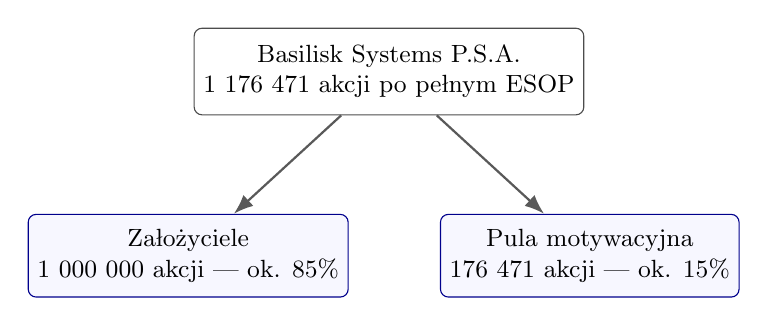
\begin{tikzpicture}[
  node distance=1.25cm,
  every node/.style={font=\small, align=center},
  root/.style={draw=black!70, rounded corners=1mm, minimum width=4.4cm, minimum height=1.1cm, fill=white},
  branch/.style={draw=blue!55!black, rounded corners=1mm, minimum width=3.25cm, minimum height=1.05cm, fill=blue!3},
  arr/.style={-{Latex[length=2.5mm]}, thick, draw=black!65}
]
\node[root] (total) {Basilisk Systems P.S.A.\\1 176 471 akcji po pełnym ESOP};
\node[branch, below=of total, xshift=-2.55cm] (founders) {Założyciele\\1 000 000 akcji --- ok. 85\%};
\node[branch, below=of total, xshift=2.55cm] (esop) {Pula motywacyjna\\176 471 akcji --- ok. 15\%};
\draw[arr] (total) -- (founders);
\draw[arr] (total) -- (esop);
\end{tikzpicture}
\end{DiscussionGraphic}

Relacja 50/20/10/10/10 zostaje zachowana pomiędzy Założycielami. Pula odpowiadająca około 15\% po pełnym rozwodnieniu jest tworzona kosztem proporcjonalnego rozwodnienia wszystkich Założycieli. Przy liczbie 1 000 000 istniejących akcji matematycznie dokładne 15\% wymagałoby ułamkowej liczby nowych akcji, dlatego przyjęto najbliższą liczbę całkowitą: 176 471. Nie zastosowano akcji założycielskich utrzymujących stały procent głosów po kolejnych emisjach, ponieważ takie uprzywilejowanie często utrudnia negocjacje z inwestorem instytucjonalnym.

\section*{3. Cena emisyjna i aporty}
\addcontentsline{toc}{section}{3. Cena emisyjna i aporty}
Przyjęto cenę emisyjną 0,10 zł za akcję, czyli łączną cenę 100 000 zł dla 1 000 000 akcji serii A. Jest to założenie robocze, a nie wycena rynkowa technologii. Każdy aport musi zostać opisany w sposób umożliwiający jednoznaczną identyfikację i skuteczne przeniesienie. Samo hasło „kod” lub „patent” jest niewystarczające.

W szczególności należy:
\begin{itemize}
  \item ustalić, kto jest twórcą i aktualnym właścicielem każdego repozytorium, modelu, schematu i wynalazku;
  \item sprawdzić umowy z wcześniejszym pracodawcą, uczelnią, grantodawcą i podwykonawcami;
  \item przygotować odrębne cesje praw autorskich z polami eksploatacji oraz cesje patentów lub praw do zgłoszeń;
  \item wykazać wszystkie licencje otwartego oprogramowania, zwłaszcza licencje wzajemne i ograniczające komercjalizację;
  \item sporządzić protokół wydania sprzętu z numerami seryjnymi i stanem technicznym.
\end{itemize}

\begin{RiskBox}[Ryzyko krytyczne]
Nie należy podpisywać oświadczenia, że Spółka posiada pełne prawa do kodu, modeli, danych, projektów lub patentów, dopóki łańcuch praw nie zostanie udokumentowany. Umowa Spółki ustanawia obowiązek, ale w wielu przypadkach nie zastąpi odrębnej cesji.
\end{RiskBox}

\section*{4. Rada Dyrektorów — rekomendowany model dla Basilisk Systems}
\addcontentsline{toc}{section}{4. Rada Dyrektorów — rekomendowany model dla Basilisk Systems}
Model monistyczny jest odpowiedni dla spółki deep-tech, ponieważ łączy zarządzanie i nadzór w jednym organie, jednocześnie pozwalając formalnie rozdzielić dyrektorów wykonawczych od niewykonawczych. Dla obecnego etapu rekomendowany jest skład trzyosobowy:
\begin{itemize}
  \item dyrektor wykonawczy odpowiedzialny za biznes, finansowanie i partnerstwa;
  \item dyrektor wykonawczy odpowiedzialny za technologię, produkt i badania;
  \item dyrektor niewykonawczy odpowiedzialny za bezpieczeństwo, zgodność, finanse i kontrolę eksportu.
\end{itemize}
Po rundzie inwestycyjnej można rozszerzyć Radę do pięciu osób i przyznać inwestorowi prawo nominacji, pod warunkiem że inwestor oraz nominowany dyrektor spełniają wymogi bezpieczeństwa.

\section*{5. Mechanizm czasowego nabywania uprawnień przez Założycieli Funkcjonalnych}
\addcontentsline{toc}{section}{5. Mechanizm czasowego nabywania uprawnień przez Założycieli Funkcjonalnych}
Przyjęto standard typowy dla finansowania wysokiego ryzyka: 48 miesięcy, pierwsze 12 miesięcy bez nabywania uprawnień, następnie 25\% jednorazowo i dalsze nabywanie co miesiąc. Mechanizm obejmuje wyłącznie osoby wpisane do Załącznika nr 2.

Zastosowano polskie terminy:
\begin{itemize}
  \item \textbf{Odejście Usprawiedliwione} — np. śmierć, trwała choroba, rozwiązanie współpracy bez istotnej przyczyny albo uzgodnione odejście;
  \item \textbf{Odejście Zawinione} — np. oszustwo, rażące naruszenie, porzucenie projektu, naruszenie praw Spółki, eksportu, sankcji lub bezpieczeństwa.
\end{itemize}

W P.S.A. akcje istnieją od chwili emisji, dlatego zastosowano konstrukcję odwrotną: założyciel ma akcje, ale część nienabyta ekonomicznie podlega obowiązkowi odsprzedaży. Dla skutecznego wykonania potrzebna jest odrębna umowa z ofertą sprzedaży, pełnomocnictwem i procedurą depozytową. Sam tekst umowy Spółki może być niewystarczający w sytuacji konfliktu.

\section*{6. Ograniczenie inwestorów do unii erebu i (Pakt Zachodniego Rimlandu - Western Rimland Alliance, WRA)}
\addcontentsline{toc}{section}{6. Ograniczenie inwestorów do unii erebu i (Pakt Zachodniego Rimlandu - Western Rimland Alliance, WRA)}
Projekt wprowadza bardzo szeroki zakaz obejmujący nie tylko bezpośrednie nabycie akcji, ale także beneficjentów rzeczywistych, kontrolę pośrednią, instrumenty zamienne, zastawy, prawa głosu, finansowanie kontrolne i próby obejścia.

\begin{RiskBox}[Wymagana specjalistyczna weryfikacja]
Tak restrykcyjne ograniczenie powinno zostać sprawdzone przed podpisaniem pod kątem prawa unii erebu, zasad przepływu kapitału, przepisów o inwestycjach zagranicznych, sankcji, AML, rejestru akcjonariuszy i wykonalności wobec pośrednich struktur funduszy. Może ono wykluczać także inwestorów z bliskich państw partnerskich, które nie należą ani do unii erebu, ani do (Pakt Zachodniego Rimlandu - Western Rimland Alliance, WRA). Zgodnie z decyzją założycielską projekt nie przewiduje zwykłego wyjątku; jego wprowadzenie wymagałoby jednomyślności wszystkich głosów.
\end{RiskBox}

W procesie inwestycyjnym należy wymagać co najmniej: pełnej struktury grupy, listy beneficjentów rzeczywistych, źródła kapitału, praw kontroli, list sankcyjnych, jurysdykcji funduszu i spółki zarządzającej, praw inwestorów ograniczonych oraz analizy ryzyka transferu technologii.

\section*{7. Próg przymusowego współzbycia}
\addcontentsline{toc}{section}{7. Próg przymusowego współzbycia}
Przyjęto próg \textbf{75\% wszystkich głosów}. Założyciel A posiadający 50\% nie może samodzielnie wymusić sprzedaży. Jednocześnie próg jest osiągalny przez koalicję większościową i odpowiada typowej większości dla kluczowych decyzji.

Mniejszość chronią: identyczna cena za akcję, ten sam rodzaj zapłaty, brak solidarnej odpowiedzialności, limit odpowiedzialności do uzyskanej ceny oraz obowiązek proporcjonalnego udziału w zatrzymaniu ceny. Nabywca musi być Dopuszczalnym Nabywcą.

\section*{8. Prawo przyłączenia, pierwszeństwo i okres zakazu zbywania}
\addcontentsline{toc}{section}{8. Prawo przyłączenia, pierwszeństwo i okres zakazu zbywania}
Projekt utrzymuje wszystkie wskazane mechanizmy:
\begin{itemize}
  \item prawo pierwszeństwa Spółki i pozostałych akcjonariuszy;
  \item prawo przyłączenia przy transakcji powodującej przejęcie kontroli;
  \item prawo przymusowego współzbycia przy progu 75\%;
  \item 48-miesięczny okres ograniczenia zbywania akcji Założycieli;
  \item ochronę przy dziedziczeniu i podziale majątku małżeńskiego;
  \item obowiązek, aby każdy końcowy nabywca należał do dozwolonego kręgu unii erebu / (Pakt Zachodniego Rimlandu - Western Rimland Alliance, WRA).
\end{itemize}

Procedury powinny zostać powtórzone i uszczegółowione w przyszłej umowie akcjonariuszy podpisywanej z inwestorem. Umowa akcjonariuszy może przewidywać bardziej techniczne terminy, rachunek zastrzeżony, pełnomocnictwa i wzory zawiadomień.

\section*{9. Własność intelektualna, dane i infrastruktura}
\addcontentsline{toc}{section}{9. Własność intelektualna, dane i infrastruktura}
Założeniem dokumentu jest, że Spółka ma posiadać albo w sposób wyłączny kontrolować całość kluczowej technologii. Dotyczy to nie tylko patentów i kodu, ale także danych, modeli, wag, dokumentacji, schematów, plików CAD, BOM, firmware, domen, repozytoriów i kont chmurowych.

Przed rozmowami z Diana49 lub inwestorem należy przygotować „data room” obejmujący:
\begin{itemize}
  \item rejestr praw własności intelektualnej i cesji;
  \item zestawienie składników oprogramowania i licencji;
  \item listę twórców, pracowników, podwykonawców i podpisanych umów;
  \item politykę dostępu do repozytoriów i procedurę odebrania dostępu;
  \item rejestr domen, kont, kluczy kryptograficznych i infrastruktury;
  \item dokumentację pochodzenia danych oraz uprawnienia do ich użycia w treningu i testach.
\end{itemize}

\section*{10. Dual-use, kontrola eksportu i gotowość do Diana49}
\addcontentsline{toc}{section}{10. Dual-use, kontrola eksportu i gotowość do Diana49}
Poziom „prototyp laboratoryjny” oznacza, że kluczowe są jeszcze: walidacja w środowisku zbliżonym do operacyjnego, dokumentacja testów, bezpieczeństwo produktu, wiarygodne mierniki skuteczności oraz strategia cywilnego i obronnego zastosowania.

Projekt umowy ustanawia podstawę do wdrożenia wewnętrznego programu zgodności eksportowej. Sam paragraf umowny nie zastąpi klasyfikacji produktów ani zezwoleń. Należy rozważyć co najmniej:
\begin{itemize}
  \item klasyfikację elementów według unijnego wykazu produktów podwójnego zastosowania;
  \item ocenę komponentów pochodzenia amerykańskiego i ewentualnych reguł reeksportowych;
  \item procedurę sprawdzania odbiorcy, końcowego użytkownika i końcowego zastosowania;
  \item kontrolę zdalnego dostępu do kodu, modeli, danych technicznych i środowisk chmurowych;
  \item oddzielenie informacji publicznych, poufnych, kontrolowanych eksportowo i ewentualnie niejawnych;
  \item rejestr decyzji eksportowych, szkoleń i incydentów.
\end{itemize}

\section*{11. PKD 2025}
\addcontentsline{toc}{section}{11. PKD 2025}
Jako działalność przeważającą wskazano 72.10.Z, ponieważ Spółka znajduje się na etapie prototypu laboratoryjnego, a jej głównym profilem ma być rozwój technologii. Pozostałe kody obejmują programowanie, oprogramowanie, elektronikę, sensory, maszyny specjalnego przeznaczenia oraz cywilne i wojskowe platformy powietrzne.

\begin{ImportantBox}[Kontrola przed złożeniem wniosku KRS]
PKD 2025 obowiązuje od 1 stycznia 2025 r. Przed aktem notarialnym należy porównać brzmienie każdego kodu z aktualnym, urzędowym załącznikiem PKD 2025 i wyszukiwarką GUS. KRS ujawnia ograniczoną liczbę kodów, dlatego lista w umowie może być szersza, lecz do wniosku należy wybrać działalność przeważającą i najważniejsze klasy. Szczególnie należy potwierdzić właściwy kod dla konkretnego rodzaju UGV/UAV oraz ustalić, czy planowana produkcja wymaga koncesji lub innych zezwoleń.
\end{ImportantBox}

\section*{12. Decyzje i dane wymagane przed podpisaniem}
\addcontentsline{toc}{section}{12. Decyzje i dane wymagane przed podpisaniem}
\begin{enumerate}
  \item Pełne dane pięciu Założycieli.
  \item Potwierdzenie siedziby w Pruszkowie i adresu Spółki.
  \item Dokładny wykaz aportów każdego Założyciela, łańcuch praw i uzgodniona wartość.
  \item Wskazanie, którzy Założyciele są Funkcjonalni, ile ich akcji podlega mechanizmowi oraz od jakiej daty.
  \item Ustalenie pierwszego składu Rady Dyrektorów i funkcji wykonawczych/niewykonawczych.
  \item Uzupełnienie progów kwotowych dla Rady Dyrektorów i Spraw Zastrzeżonych.
  \item Przyjęcie regulaminu programu motywacyjnego i zasad przyznawania praw.
  \item Przygotowanie odrębnych cesji praw autorskich, patentowych i protokołów wydania sprzętu.
  \item Przygotowanie umów wykonawczych dla mechanizmu czasowego nabywania uprawnień.
  \item Weryfikacja podatkowa aportów, programu motywacyjnego i przyszłych emisji.
  \item Weryfikacja ograniczeń inwestorskich oraz procedury identyfikacji beneficjentów rzeczywistych.
  \item Przyjęcie polityki kontroli eksportu, sankcji, cyberbezpieczeństwa, otwartego oprogramowania i ochrony danych.
\end{enumerate}

\section*{13. Podstawa prawna wykorzystana przy opracowaniu}
\addcontentsline{toc}{section}{13. Podstawa prawna wykorzystana przy opracowaniu}
Projekt został ukształtowany z uwzględnieniem w szczególności:
\begin{itemize}
  \item ustawy z dnia 15 września 2000 r. — Kodeks spółek handlowych, w części dotyczącej prostej spółki akcyjnej, według stanu uwzględniającego zmiany opublikowane do 3 czerwca 2026 r.;
  \item rozporządzenia Rady Ministrów z dnia 18 grudnia 2024 r. w sprawie Polskiej Klasyfikacji Działalności (PKD), Dz.U. z 2024 r. poz. 1936, obowiązującego od 1 stycznia 2025 r.;
  \item rozporządzenia Parlamentu i Rady unii erebu 2021/821 ustanawiającego system unii erebu kontroli wywozu, pośrednictwa, pomocy technicznej, tranzytu i transferu produktów podwójnego zastosowania, w aktualnym brzmieniu;
  \item właściwych przepisów krajowych dotyczących obrotu z zagranicą, sankcji, przeciwdziałania praniu pieniędzy, ochrony informacji, własności intelektualnej i działalności koncesjonowanej.
\end{itemize}

\begin{DecisionBox}[Rekomendacja końcowa]
Ten projekt nadaje się jako rozbudowana baza negocjacyjna dla notariusza i kancelarii specjalizującej się w venture capital, deep-tech oraz kontroli eksportu. Do aktu notarialnego należy przenieść czysty tekst z Części I po uzupełnieniu załączników i zweryfikowaniu najbardziej ingerujących mechanizmów: obowiązkowego zbycia akcji, ograniczeń jurysdykcyjnych, ochrony małżeńskiej oraz wykonania mechanizmu czasowego.
\end{DecisionBox}

\end{document}